\chapter{Systems}
\label{chapSystems}

\section{Simulator}

\subsection{N-Process Machines}
\label{secSystemNPM}

Part of the motivation for this work is to examine fault tolerance on large systems, specifically cloud systems.
To do this we shall use an abstraction from specific systems and talk about N-Process Machines (NPM).
An NPM is a generalisation of cloud-like computers which is more useful when examining theoretical aspects of FT, as we are.
The name is drawn from the theoretical machine's nature, the NPM is simply $n$ connected processes which run independently.

Importantly this abstraction better represents cloud computers (than, say, multicores or cell processors) because it makes no assumption on homogeneity.
Assignment and synchronisation problems can be simplified slightly for more conventional multicores and unicores, since the processing power of the individual elements is identical.
To an extent this is true of some cell architectures, which provide multiple CPUs which are largely identical, though with different speeds.
In the case of the cell-like machines, the speed of processor $i$ is some constant factor different from that of $j$ for any computation.
However the NPM does not make these assumptions, and better represents systems composed of large numbers of heterogeneous computers.
For this machine any computation may have a different running time on any process, and these may be completely independent.
That is, if task $i$ runs in time $a$ on processor $x$ and $b$ on $y$, and task $j$ runs in time $c$ on $x$, then $j$ need not run in time ${b}\over{a}c$ on processor $y$.
These running times are typically represented as a matrix; for more detail see Chapter \ref{chapModel}.
We shall use $\invoke{a}{p}$ as shorthand for the cost of invoking actor $a$ on processor $p$.

The same disparity is allowed in the case of process communication.
Again, it would be simpler in the case of unicore or multicore machines, which have no communication or identical communication costs between processors.
However, in the case of distributed cloud systems, the communication channels could be anything from optical fibre to wireless.
Processes are allowed to make connections and send data between each other, and this amount may vary for every actor and processor pair.
To an extent, the cost of setting up the network (that is, establishing communication channels) is dominated by the cost of communication during execution, since SDF programs are designed to run indefinitely.
We shall use $\commu{a_1}{a_2}{p_1}{p_2}$ as shorthand for the cost of allowing actors $a_1$ and $a_2$ to communicate if they are assigned to $p_1$ and $p_2$ respectively.

Finally these machines are not expected to have in-built control mechanisms.
That is, for simplicity we are allowed to assume that initial data and code is placed on the right processor before execution ``magically'', as we only care about the system during execution.
In our case it is necessary to consider the implications of having to re-assign and initialise computers that crash during execution, details on how this is done are explained in Section \ref{secSystemFault}

\subsection{High Level Purpose}

The simulator is designed to execute and analyse SDF programs on the NPM described above.
For the remainder of this thesis we shall call it the SDFSimulator.
The simulator is written in Java standard edition, though makes use of external libraries for Integer Linear Programming provided by the GLPK, with integer linear programmes written in AMPL.

In broad terms the SDFSimulator exists to examine the resilience of SDF programs under the various FT mechanisms as well as varying fault-conditions.
By design the simulator can handle the execution, in theory, of artificial SDF graphs (which do not perform real computation) as well as functional graphs.
In this case, the actor-code is written in Java by extending the inbuilt actor classes.
These functional programs also can send data to others using FIFO buffers (java.util.queue), however since it is a simulator these buffers are only on the local machine and real network communication does not take place.

Given the simulated nature of the NPM, the assignment of actors is of some importance.
The SDFSimulator assigns actors to processors, which are represented by Java Threads.
These actors are executed multiple times, either with real computations, or real delays, or simply simulated delays.
Optimisations for the execution schedule are outside the scope of this work, so actors will execute if there are enough tokens available and they have not already exceeded their steady-state repetitions.

Most importantly, the simulator records metrics and statistics from the execution of the program.
This information will be used to evaluate the performance of the FT mechanisms, and so the information gathered is focused on this task.
Section \ref{secSystemStatistics} provides more detail on the information that is recorded by the Simulator.

\subsection{Main Components}
\label{secSystemComponents}

\begin{figure}
\begin{center}
	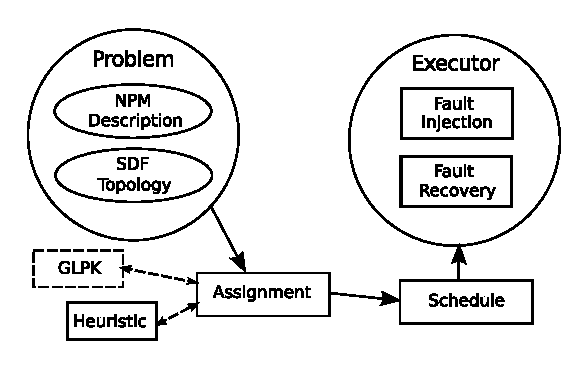
\includegraphics[width=12cm]{figures/sysDiagram.eps}
\caption{A diagram showing the interactions between the main parts of the SDFSimulator}
\label{figSysDiag}
\end{center}
\end{figure}

Figure \ref{figSysDiag} shows a diagram of the major components of the SDFSimulator.
The dashed arrows refer to external program calls.
The dashed box refers to a program not written for this thesis.

The first stage of the SDFSimulator is assignment.
In an actual distribution the assigner would be largely identical to this one, since it assigns for real NPMs, which the simulator models.
Assignment begins with calculating an SDF graph's repetitions vector, which gives us better estimates on bandwidth and processing requirements.
For simplicity, actors are not fissed onto different processes, which means their processing requirements are multiplied by their repetitions per steady-state schedule.
These estimates (bandwidth and computation requirements) are paired with an NPM specification.
The specification contains details on a concrete instance of an NPM, which the program is expected to run on, such as inter-process bandwidth costs or limitations, and the clock speed or rates per cycle for each of the processes.
For experimentation purposes many specifications are tested on a single SDF program.
The estimated costs and the specification together form an instance of an assignment problem.
The details of the assignment problem (including its complexity) have been discussed in Chapters \ref{chapModel} and \ref{chapHardness}.
Our simulator uses various methods to determine assignment from the problem.
Optimal assignment can be found using a call to the external GLPK suite or using brute force in the case of small SDF graphs (less than roughly 20 nodes).
For larger graphs, the simulator can be told to assign at random or using a greedy heuristic.
Again the tests being run will determine which assignment protocol is used.

Once assigned, an invocation schedule can be formulated.
The schedule is the order in which actors are invoked in the simulator.
Formulation of schedules is an area of research interest in its own right, however this thesis is not concerned with optimisations for buffer requirements.
It is of some interest, however, whether the schedule can affect the FT of the computation.
To this end the exact scheduling algorithm is chosen differently for different tests, where simple scheduling is done based on availability, but more realistic scheduling involves random or dynamic selection from a pool of idle actors.
These schedules may also be interleaved and variable over multiple steady states.

Finally the program is handed to an executor.
This module is responsible for invoking actors according to the schedule, recording the statistics used for analysis and injecting, and recovering from, faults.
Fault injection is described more thoroughly in Section \ref{secSystemFault}, as well as the exact nature of the recovery/resilience systems.
The executor attempts to follow the order in the schedule, however faults may cause this to be impossible, in which case it records the problem and restarts the simulation.
It also orchestrates the FIFO buffers used by each actor for inter-process communication, which allows it to strategically fault them by withholding the buffer at times, which would be much like cutting an Ethernet cable in a cloud system.
In a way, the executor is not responsible for fixing all faults.
Faults must be correctly identified by the processes themselves (which the executor simulates), and there is no overarching control program for real cloud systems to defer this to; again, see Section \ref{secSystemFault} for more details.

\section{Fault Analysis}
\label{secSystemFault}
\subsection{Checkpointing}

The checkpointing FT mechanism is designed to recover either individual actors or the entire network in the event of a fault.
Periodically during execution the processes in the NPM write their state (RAM in a conventional machine) to non-volatile memory.
In the event of a fault, the system rolls back to the last successful state.
This methodology makes the assumption that the faults occur independently of the system's state, or that persistent bugs will not cause faults later down the system's pipeline.
This work will assume that actor code is bug-free, and that actors are able to deal sensibly with bad data.

The frequency of checkpointing facilitates a tradeoff between performance and robustness.
If we checkpoint frequently we expend a lot of computation on the checkpointing itself, however our backups of the system are more up-to-date.
On the other hand rarer checkpointing saves computation on checkpointing itself but means that in the event of a fault, the system-wide rollback will cause a lot of wasted computation.
The SDFSimulator takes the simple approach to checkpointing and saves state once every steady state execution.
The expected costs of using checkpointing is calculated in Chapter \ref{chapModel} using the presumption of one checkpoint per steady-state iteration.

The checkpointing must be able to recover the system to a working state, which means recording sufficient information.
This raises a minor issue regarding how to correctly save the state of stateful actors.
Naively we would have to record the internal memory of each individual actor, as well as the content of all memory buffers (used for inter-actor communication) when checkpointing.
However, with simple modifications to the code, any stateful actor can be converted to a stateless one with a communication channel to itself.
This simplification allows us to ignore the existence of stateful actors and only record the content of memory buffers.

Detection and recovery form an important part of the simulation.
First, the simulator cannot use its oracular powers of knowing when a fault has occurred.
The worker-threads described in Section \ref{secSystemComponents} can record faults in the other threads both upstream and downstream from themselves.
Actors upstream which reside on faulting processors do not produce tokens for the downstream actors, which leads to starvation.
The simulator, by means of a steady state schedule, can make the guarantee that any invoked actor should have sufficient tokens to execute, however this is not the case when faulting actors fail to fill those buffers.
Faults downstream break communication protocols, or put simply, faulting actors do not acknowledge TCP packets within a set time after the communication.
This method, called {\em timeout} is used commonly to detect interrupted connections in TCP.
For simplicity, we can think of the consuming actor as hosting a connection and the producing actor as making the remote connection, which means we would expect an acknowledgement from the host when we send data.
This behaviour is modelled in the simulator.

Once detected, faults must be recovered from, which involves rolling back to the last checkpoint.
First the faulting computer must be restarted with some overhead, this is modelled by creating a new Java thread to take over the job of the faulted one.
Next the new thread must be brought to the correct state.
In a real system the restarted computer would have to read the last saved state from the checkpoint database, the simulator instantiates and fills the FIFO buffers used to represent communication buffers.
Finally the non-faulting machines must roll-back as well, in much the same way as the faulting one.
A slightly more complicated variation would be to have the checkpoints stored away from the machine whose state they record.
This would allow non-faulting computers to virtualise and recover the tasks that the faulted machine would perform, even in the event that the machine is completely unrecoverable.

\subsection{Replication}

Replication FT tries to ensure the continued execution of parts of the system despite the failure of individual components.
Before the network is executed or even assigned, each actor is duplicated several times, all of which perform the same computation.
During assignment, we ensure that duplicates do not run on the same processor.
This means that if one processor dies, there are still duplicates of the actors on that processor running elsewhere.
Under pathological cases this mechanism does not guarantee fault-less execution.
To meet this guarantee requires recovery schemes which this thesis does not discuss.
Though the system failing requires the statistically improbable faulting of all computers hosting duplicates of the same actor.
As a result, this method is only viable due to over-provision of processors and having many duplicates.

One important consideration with duplicates is how to facilitate communication.
There are several ways we can handle this, one is to not duplicate communication.
Under this scheme all actors are duplicated the same number of times and communicate in parallel only with the correct duplicate.
In effect we treat the entire SDF computation as a single program and run it several times in parallel.
This causes a linear increase in communication volume, however the entire duplicate network can be broken by faulting a single actor.
This means the system is only more resilient (the probability of failing is lowered) by a relatively small amount.
We can make a tradeoff on communication to gain significantly higher resilience, by making each duplicate send data to all the duplicates of the next.
This causes quadratic increase in the communication volume (so three duplicates cause nine times the volume), however now the network will function so long as at least one duplicate of every actor remains, a significant improvement.
A more thorough description of the mathematics behind this is presented in Chapter \ref{chapModel}.
Our simulator uses this method for comparison against the checkpoint recomputation.

Fault detection and recovery is handled very differently with replication-type FT.
Namely, detection occurs on a per-actor basis and recovery does not occur at all.
Each actor can examine the several supposedly identical duplicate tokens handed to it by each duplicate of its predecessor.
In the event that one of its predecessors stops providing tokens we can conclude that the processor died, however this actor simply continues with the inputs given by the other duplicates.
Similarly if a processor topologically below this one stops sending acknowledgements, an actor can presume it has faulted and stop trying to send tokens to it.
This mechanism also allows actors to examine token correctness.
In the event that the actor receives tokens with differing content from its duplicate predecessors, it can, given enough duplicates, decide to ignore the output from faulting channels.
This behaviour provides some defence against compromised systems and malicious attack, requiring that all duplicates are compromised in an identical fashion.
For this thesis we assume no attempt is made to recover when a faulty processor is detected.
In practice it would be possible to recover by injecting the state of an actor's duplicates into the faulted one.
However for simplicity our simulator does not perform this recovery.

\subsection{Fault Injection}

Naturally, the SDFSimulator must also simulate faults in a real cloud machine.
For simplicity we shall exclude data errors, such as those caused by hardware imprecision for floating point computations in GPUs, and focus on network-stability-threatening faults.
Faults of this kind occur in the major hardware components of the system, CPUs, disk, Ethernet cables etc.
The results are either that a computer in the network crashes and stops working, or that communication between nodes is broken where wires have excessive interference or breaks.
In the simulator the computers are replaced with worker threads and the wires by FIFO buffers, so they must become the targets of our simulated faults.
Wiring faults, or communication faults, are simulated by blocking writes to the FIFO buffers.
This will cause both the producing and consuming actors to flag the other as faulted (the consumer starves and the producer receives no acknowledgement).
This is the expected behaviour, since the inability of two computers to communicate with each other makes them both unsuitable for use.
Computer faults are simulated by terminating worker threads.
This will cause actors upstream and downstream of the fault to flag it.
Again such behaviour is expected.

The frequency of faults is dealt with on a per-experiment basis.
Experiments which emulate real computations are difficult to run on the simulator, as they require thousands of worker threads each with simulated up-times of $10^5$ hours.
The probability of faults is skewed to greater frequency so as to examine the effects of multiple faults on the network.
Faults can also be scripted to occur at certain times or on certain threads, again this is used for experimentation and reproducibility reasons.
We accept the slightly unrealistic frequency of faulting in these cases because we are not concerned in this thesis with the vast majority of real-world computations which run flawlessly.
This work aims to analyse the resilience of fault tolerance mechanisms to faults and their overhead costs, the question of whether these tradeoffs are acceptable given the frequency of faults is debatable.

\section{Statistical Measurements}
\label{secSystemStatistics}
\subsection{Recorded Figures}

Recorded figures includes actual data from the execution of the SDF network in the simulator.
These recoded figures are important in their own right, but they are also used to estimate the metrics in Section \ref{secSystemMetrics}.

\begin{itemize}
	\item {\em Token counts} simply record the number of tokens passed around the SDFSimulator.
			These counts do not actually indicate the volume of data transferred, however they are useful for judging the overheads associated with the different FT mechanisms.
			This includes every FIFO buffer and every token passed between every pair of actors.
	\item {\em Invocation counts} record the number, and order, of actor invocations.
			Invocation count is not particularly interesting except again in analysing how the FT mechanisms affect the system.
	\item {\em Fault counts} are recorded to ensure reproducibility and fairness in experiments.
			This figure also records where and when the fault was simulated, and if/how it was detected by the network.
	\item {\em Recovery time} is recorded to put some real world figures on the overheads of recovery.
			Like the other recorded timings, this time does not represent real-world numbers, as it all takes place in a simulator.
	\item {\em Steady-State execution time} is used in conjunction with the recorded recovery time.
			Though they are both recording times in a simulator, and therefore inaccurate, together they can be used to gauge the relative difference in times associated with a recovery and with a normal execution.
	\item {\em Average execution time} is similar to the above but accounts for disparity in the execution times of different steady-state invocations.
\end{itemize}

\subsection{Metrics}
\label{secSystemMetrics}

Not all real world figures can be recorded in the simulator.
Importantly the major indicators, bandwidth and makespan, must be estimated using combinations of the above recordings and some assumptions.

\begin{itemize}
	\item {\em Makespan} is a function of invocation counts and assumed execution times for each actor.
			Understandably these times must be estimated using real world tests and knowledge of the target architectures.
			During the assignment stage estimates of these times are required anyway, so it is reasonable to assume that the simulator can make use of them.
	\item {\em Bandwidth} is a function of token counts and assumed token sizes, as well as some communication overheads.
			Again this estimate requires some knowledge of the target system to account for the overheads and again this knowledge had to be available to assign the processors, so we are allowed to make use of it here.
	\item {\em Communication time} is similar to bandwidth, it must be estimated using the bandwidth estimate and communication throughput figures.
			Unsurprisingly this information was required before we assigned actors to their processors so using it to estimate communication time is not unreasonable.
\end{itemize}

\noindent
These metrics make use of some assumptions about the system that are broadly reasonable.
The precise nature of the assumptions will vary depending on the experiment being run.

\section{Working Example}

This section describes how the simulator works using our bitonic sort example from Chapter \ref{chapExample}.

\subsection{Automatic Generation}

The first step is to generate an SDF graph for bitonic sorting.
As stated in Chapter \ref{chapExample} we generate sorting networks to handle the sorting of as many items as we need.
We do this in isolation from the simulator, and generate a description of all the network nodes and the channels between them.
The actual executing actor code is included in this description, which is given to the simulator to run.

The simulator does some of the automatic generation for us.
We know, for example, that all actors in this network are identical, so we can tell the simulator to give them unit invocation costs.
The Input and Output nodes are not really meant for analysis, so we can ignore them by giving them zero invocation costs.
Each channel carries a single token per steady-state invocation, so we can give every channel unit communication cost.

In order to fully exploit parallelism in this sorting network we must simulate sufficient computers.
The simulator can pretend to have computers based on an arbitrary specification of the NPM, however, for testing purposes we simply tell it to randomly generate some reasonable computers.
These random computers have roughly equal processing time, with costs based on a random normally distributed variable.
Since these costs are artificial anyway this is an acceptable shortcut, though the SDFSimulator can be given specifications based on real cloud systems when necessary.

\subsection{Assignment}

To begin assigning actors to processors the simulator creates the costs matrices for invocation and communication (See Section \ref{secSystemNPM}).
Our example is using a randomly generated cloud machine specification and unit costs for actors and communication, so we would expect to see a reasonably even spread of random values in these matrices.

For a real assignment we would use our AMPL model or a heuristic to determine the assignment.
To use the GLPK we write these matrices to a .dat file and run \verb=glpsol= on this data using the model described in Chapter \ref{chapModel}.
Once solved we read in the assignment from the output of \verb=glpsol=.
However, since we know that all actors are the same, and all communicating channels carry the same information, we can simplify the assignment process by spreading actors evenly over the computers.
Assignment done manually in this way does not affect the later stages of the simulation, however if replication FT is being used then we must ensure the non-overlapping duplicates constraint is upheld.

Once assigned, the simulator spawns a worker thread for each of its actors (or duplicates) and places them in the work queue.
The worker thread is also told how many times each actor should execute per steady state invocation.
Finally, a FIFO buffer is made for each communication channel.
These buffers are stored as class wide variables, so all worker threads can access them.
If applicable, the initial delays for the network are injected into the right buffers.

\subsection{Execution}

The executor now begins the process of allowing worker threads to run.
We begin by performing quick initialisation for our network by saturating it (see Section \ref{BACK_SYNC}).
The process is quite simple: while a channel whose producer can execute is not saturated, execute the producer.
Not all networks are able to be saturated in this way, however our example is so the simulator is told to do so.

Once saturated, each worker thread can execute its actors in any order with any interleaving, so long as they halt after each steady-state execution.
The executor gives the instruction for all workers to proceed through a single steady-state.
To do this, each worker executes its actors in any order, in our case each actor will be executed once.
For networks which are not amenable to saturation, the execution schedule is based on availability, that is, a node executes if there are enough tokens in its input channels to do so and it has not already exceeded the repetition amount.

The execution of a single actor is based on the code we write for them.
For the bitonic sort, the input node generates a new set of items to be sorted.
The output node reads a set of items and ensures they are sorted.
The intermediate nodes read one token from each of their two input channels, then write the lesser token to their ``upper'' channel and the greater to their ``lower'' channel.
Reading and writing to channels involves making a call to the executor to enqueue or dequeue a token in the right FIFO buffer.
The executor may refuse to do this if it is simulating a wire failure or the processor at the ``end'' of that channel is supposed to have faulted.
This continues possibly indefinitely.

\subsection{Fault Analysis}

During execution we inject faults, and how our working example responds will depend on the fault and the kind of FT mechanism being used.
As has been mentioned previously, faults come in two main varieties: wire failures and computer failures.
When a wire failure is being simulated, the executor will refuse to write tokens to the broken channel, however, it will still read tokens from it until there are none, when it starts returning null.
The executor refusing to write emulates timeout detection in the simulator where no low-level communication actually occurs.
When an actor suspects a wire failure has occurred, it flags this by calling method on the executor, providing the processor it suspects is faulty as an argument.
Computer failures are simulated by terminating the worker thread executing that process, again the executor will refuse to write tokens if the process at the end of the channel is supposed to be dead.
The faults are flagged by the actors in the same way as wire faults.

If our example is using a checkpoint recovery mechanism, then it must try to recover.
We presume that after each steady state invocation, the actors were writing the contents of those memory buffers from which they consume to disk.
After the fault is discovered, a call is made to the executor to spawn a new worker thread.
The contents of disk are read and the last successful state is retrieved and injected into the worker thread.
Finally the checkpointed contents of disk are read by every other thread and the whole network rolls back.
Once rollback is finished an actor on the recovered process will call a method on the executor to indicate the computation can restart.

If our example is using a replication tolerance mechanism, then our simulator has no mechanism for actual recovery.
However, our actor executions will be slightly different.
Each actor is encased in a wrapper which performs the fault detection and token duplication tasks.
These wrappers are themselves an extension of the inbuilt Actor class, and so are invisible to the simulator itself.
The wrappers receive multiple tokens for each logical channel they have, they pick one of those and use it as input to the actor they encapsulate, that actor's outputs are read, duplicated, and sent to all the duplicates of the actor at the logical end of that channel.
These wrappers also flag the executor when faults are detected using the same procedure described above.
